
\documentclass[pdf, unicode, 12pt, a4paper,oneside,fleqn]{article}
\usepackage{graphicx}
\graphicspath{{img/}}
\usepackage{log-style}
\begin{document}

\begin{titlepage}
    \begin{center}
        \bfseries

        {\Large Московский авиационный институт\\ (национальный исследовательский университет)}
        
        \vspace{48pt}
        
        {\large Факультет информационных технологий и прикладной математики}
        
        \vspace{48pt}
        
        Лабораторная работа \textnumero 4 по курсу \enquote{Операционные системы}

        \vspace{48pt}

        Освоение принципов работы с файловыми системами. 
        
        Обеспечение обмена данных между процессами посредством технологии <<File mapping>>.
    \end{center}
    
    \vspace{140pt}
    
    \begin{flushright}
    \begin{tabular}{rl}
    Студент: & П.\,Ф. Гришин \\
    Преподаватель: & Е.\,С. Миронов \\
    Группа: & М8О-201Б-21 \\
    Вариант: & 16 \\
    Дата: & \\
    Оценка: & \\
    Подпись: & \\
    \end{tabular}
    \end{flushright}
    
    \vfill
    
    \begin{center}
    \bfseries
    Москва, \the\year
    \end{center}
\end{titlepage}
    
\pagebreak

\section{Постановка задачи}

Составить и отладить программу на языке Си, осуществляющую работу с процессами 
и взаимодействие между ними в одной из двух операционных систем. В результате работы 
программа (основной процесс) должен создать для решения задачи один или несколько 
дочерних процессов. Взаимодействие между процессами осуществляется через системные 
сигналы/события и/или через отображаемые файлы (memory-mapped files).

Необходимо обрабатывать системные ошибки, которые могут возникнуть в результате работы.

Родительский процесс передает команды пользователя дочернему процессу. Дочерний процесс 
принеобходимости передает данные в родительский процесс. Результаты своей работы дочерний
процесс пишет в созданный им файл.

Правило проверки: строка должна оканчиваться на «.» или «;»

\begin{figure}[htp]
    \centering
    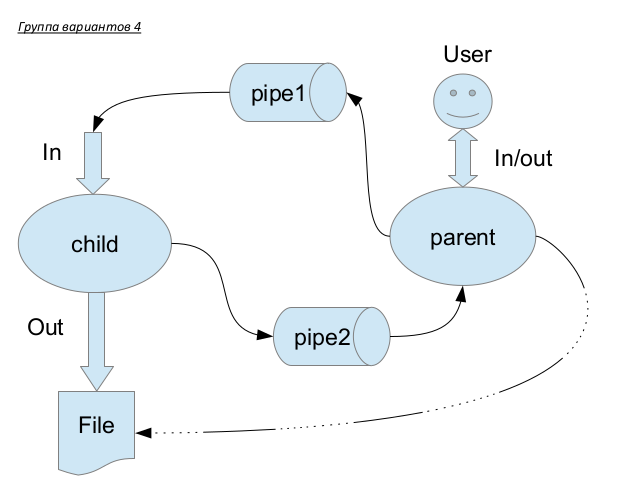
\includegraphics[width=11cm]{os2.png}
    \caption{Структура программы}
    \label{fig:os2}
\end{figure}

\section{Сведения о программе}

Программа написанна на Си в Unix подобной операционной системе на базе ядра Linux.
При компиляции следует линковать библиотеки -lpthread и -lrt.
В программе создается дочерний процесс, данные в который передаются с помощью shared memory.

Дочерний прочесс принимает строку и проверяет подходит ли данная строка в соответствии с правилом, ответ записывая в файл. Имя файла задается пользователем.

Родительский процесс считывает вводные данные у пользоветеля и пердет их дочернему процессу через отброженный участок памати shared memory.

Программа завершает работу при окончании ввода, то есть нажатии CTRL+D.

\section{Листинг программы}

{\large\textbf{pc.c}}

\begin{lstlisting}[language=C]
#include "library.h"
void handle_error(bool expr, char* msg){
    if (expr){
        perror(msg);
        exit(-1);
    }
}

void clean(char* str){
    for (int i = 0 ; i < strlen(str); ++i){
        if (str[i] == '\n'){ str[i] = '\0'; }
    }
}

bool StrLength(char* str) {
    return str[strlen(str) - 1] == '.' || str[strlen(str) - 1] == ';';
}

int ParentRoutine(char* nameF){
    FILE* file = fopen(nameF, "r");
    handle_error(file == NULL , "open error");

    const char* SOURCE_SEMAPHORE_NAME = "source_sem";
    const char* RESPONSE_SEMAPHORE_NAME = "response_sem";

    sem_unlink(SOURCE_SEMAPHORE_NAME);
    sem_unlink(RESPONSE_SEMAPHORE_NAME);

    const char* SOURCE_NAME = "source_shm";
    const char* RESPONSE_NAME = "response_shm";
    const int SIZE = 4096;

    shm_unlink(SOURCE_NAME);
    shm_unlink(RESPONSE_NAME);

    int source_fd = shm_open(SOURCE_NAME, O_RDWR | O_CREAT, 0644);
    int response_fd = shm_open(RESPONSE_NAME, O_RDWR | O_CREAT, 0644);
    handle_error(source_fd == -1 || response_fd == -1, "can't open shared memory object");

    handle_error(ftruncate(source_fd, SIZE) == -1 ||
                 ftruncate(response_fd, SIZE) == -1,
                 "can't resize shared memory object");

    void* source_ptr = mmap(NULL, SIZE, PROT_READ | PROT_WRITE, MAP_SHARED, source_fd, 0);
    void* response_ptr = mmap(NULL, SIZE, PROT_READ | PROT_WRITE, MAP_SHARED, response_fd, 0);
    handle_error(source_ptr == MAP_FAILED || response_ptr == MAP_FAILED, "can't mmap shared memory object");

    sem_t* source_semaphore = sem_open(SOURCE_SEMAPHORE_NAME, O_RDWR | O_CREAT, 0644, 0);
    sem_t* response_semaphore = sem_open(RESPONSE_SEMAPHORE_NAME, O_RDWR | O_CREAT, 0644, 0);
    handle_error(source_semaphore == SEM_FAILED ||
                 response_semaphore == SEM_FAILED,
                 "can't open semaphore");

    pid_t pid = fork();
    handle_error(pid == -1, "fork error");

    if (pid == 0){

        sem_wait(source_semaphore);
        char* name = source_ptr;
        int output_fd = open(name, O_WRONLY | O_CREAT, 0644);
        char* file_error = "0";
        if (output_fd < 0){ file_error = "1"; }
        strcpy(response_ptr, file_error);
        sem_post(response_semaphore);

        sem_wait(source_semaphore);
        char* str = source_ptr;
        while (strcmp(str, "\0") != 0){
            char* error = "0";
            if (StrLength(str)){
                write(output_fd, str, strlen(str) * sizeof(char));
                write(output_fd, "\n", sizeof "\n");
            } else {
                error = "1";
            }
            strcpy(response_ptr, error);
            sem_post(response_semaphore);
            sem_wait(source_semaphore);
            str = source_ptr;
        }

    } else {

        const int parent = getpid();
        printf("[%d] Enter the name of file to write: ", parent);
        fflush(stdout);
        char name[256];
        fscanf(file, "%s", name);
        clean(name);
        printf("%s\n", name);
        strcpy(source_ptr, name);
        sem_post(source_semaphore);

        sem_wait(response_semaphore);
        if (strcmp(response_ptr, "1") == 0){
            close(source_fd);
            close(response_fd);
            shm_unlink(SOURCE_NAME);
            shm_unlink(RESPONSE_NAME);
            munmap(source_ptr, SIZE);
            munmap(response_ptr, SIZE);
            sem_destroy(source_semaphore);
            sem_destroy(response_semaphore);
            sem_unlink(SOURCE_SEMAPHORE_NAME);
            sem_unlink(RESPONSE_SEMAPHORE_NAME);
            handle_error(true, "file error");
        }

        char str[256];
        printf("[%d] Enter string: ", parent);
        fflush(stdout);
        while (fscanf(file, "%s", str) != EOF){
            printf("%s\n", str);
            clean(str);
            strcpy(source_ptr, str);
            sem_post(source_semaphore);
            sem_wait(response_semaphore);
            char* error = response_ptr;
            if (strcmp(error, "1") == 0){
                printf("Error: \"%s\" is not valid.\n", str);
            }
            printf("[%d] Enter string: ", parent);
            fflush(stdout);
        }

        printf("\n");
        fflush(stdout);

    }

    close(source_fd);
    close(response_fd);
    shm_unlink(SOURCE_NAME);
    shm_unlink(RESPONSE_NAME);
    munmap(source_ptr, SIZE);
    munmap(response_ptr, SIZE);
    sem_destroy(source_semaphore);
    sem_destroy(response_semaphore);
    sem_unlink(SOURCE_SEMAPHORE_NAME);
    sem_unlink(RESPONSE_SEMAPHORE_NAME);
    fclose(file);
}
\end{lstlisting}

\section{Демонстрация работы программы}

\begin{alltt}
gpavel@gpavel-HP-Pavilion-Gaming-Laptop-17-cd1xxx:~/Desktop/OS/lab4$ ./Lab4 
test.txt
[43971] PARENT. Enter the name of file to write: OutputFile.txt
[43971] PARENT. Enter string: FirstTest.
[43971] PARENT. Enter string: False
[43971] PARENT. Error: "False" is not valid.
[43971] PARENT. Enter string: CCCCCCCCCCCCCCCCCCC.
[43971] PARENT. Enter string: End;
[43971] PARENT. Enter string: ...........................a
[43971] PARENT. Error: "...........................a" is not valid.
[43971] PARENT. Enter string: wave...;
[43971] PARENT. Enter string: wrongString
[43971] PARENT. Error: "wrongString" is not valid.

[43971] PARENT. Enter string: 
gpavel@gpavel-HP-Pavilion-Gaming-Laptop-17-cd1xxx:~/Desktop/OS/lab4$ 

\end{alltt}

\pagebreak

\section{Вывод}

Взаимодействие между процессами можно организовать при помощи каналов, сокетов и отображаемых
файлов. В данной лабораторной работе был изучен и применен механизм межпроцессорного взаимодействия 
\--- file mapping. Файл отображается на оперативную память таким образом, что мы можем взаимодействовать
с ним как с массивом.

Благодаря этому вместо медленных запросов на чтение и запись мы выполняем отображение файла в
ОЗУ и получаем произвольный доступ за O(1). Из-за этого при использовании этой технологии межпроцессорного
взаимодействия мы можем получить ускорении работы программы, в сравнении, с использованием каналов.

Из недостатков данного метода можно выделить то, что дочерние процессы обязательно должны знать
имя отображаемого файла и также самостоятельно выполнить отображение.

\end{document}

